\subsection{Models}
The model classes in the system define the data structures of the different model components (see \autoref{sc:model_component}). These all inherit from a general abstract \textit{Model} class which dictates that certain information must be made available in the concrete models, such as ID in the database, \textit{Created\_At} and \textit{Updated\_At} (see \autoref{fig:ModelAbstractClass}).

\begin{figure}[H]
    \centering
    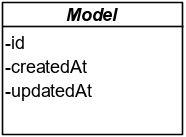
\includegraphics[width=0.2\textwidth]{figures/Implementation/Model.png}
    \caption{Overview of the model class}
    \label{fig:ModelAbstractClass}
\end{figure}

The system contains models for the following elements: \textit{Asset}, \textit{Tag}, and \textit{User}. These are the most essential and relevant models, and have been described in this subsection. 
\par
\textit{Asset} and \textit{Tag} both include fields and inherit from the \textit{FieldContainer} class. Because of this, the \textit{Field} class will also be described as it is essential for the understanding of the \textit{Asset} and \textit{Tag} classes. 